\chapter{Конструкторская часть}

\section{Процесс обучения}

\begin{figure}[H]
    \centering
    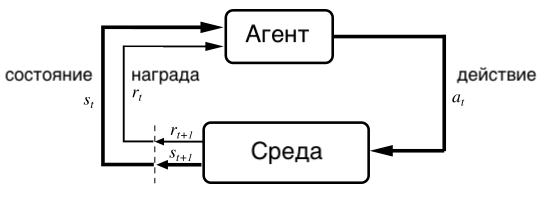
\includegraphics[width=1\textwidth]{C:/MGTU/baseAI/lr12/lr12/bag/report/images/scheme.png}
    \caption{Цикл обучения с подкреплением}
\end{figure}
Процесс обучения начинается с получения информации о состоянии $s_t$ из среды. 
Основываясь на этом состоянии, агент выполняет дейсвтие $a_t$, тем самым среда перемещается в новое состояние $s_{t+1}$.
Среда даёт вознаграждение агенту $r_{t+1}$. Агент использует вознаграждение как сигнал для корректировки действий,
стремясь максимизировать награду.

\section{Описание среды AdroitHandHammer-v1}
AdroitHandHammer-v1 -- это среда для обучения с подкреплением, являющаяся частью библиотеки gymnasium\_robotics и основанная на симуляторе MuJoCo \cite{lib:gymnasium_robotics}.

Среда предоставляет возможности:
\begin{itemize}
    \item наблюдения:
    \begin{itemize}
        \item положения и ориентации суставов роботизированной руки (24 степени свободы * 3 значения (синус, косинус, угловая скорость) = 72 значения);
        \item положения молотка в трехмерном пространстве (3 значения);
        \item положения гвоздя в трехмерном пространстве (3 значения);
        \item линейной и угловой скорости молотка (6 значений);
        \item расстояния от головки молотка до шляпки гвоздя (3 значения);
        \item вектора, указывающего направление от головки молотка до шляпки гвоздя (3 значения);
        \item состояния гвоздя (положение относительно доски, 2 значения);
    \end{itemize}
    \item действия, управляя 24 степенями свободы роботизированной руки, задавая крутящий момент для каждого сустава;
    \item награды:
    \begin{itemize}
        \item разреженной, когда агент получает награду, только если гвоздь полностью забит;
        \item плотной, когда агент получает награду, основанную на расстоянии между головкой молотка и шляпкой гвоздя, а также на прогрессе забивания гвоздя; 
    \end{itemize}
    \item условия завершения, когда эпизод завершается, если гвоздь полностью забит или по истечении максимального количества шагов;
    \item начальное состояние, когда роботизированная рука находится в начальном положении, молоток находится в "ладони", а гвоздь частично вбит в доску;
    \item данные, собранные с помощью различных политик (в том числе экспертных и случайных).
\end{itemize}

\section{Общий ход алгоритма}

Процесс обучения модели машинного обучения можно разделить на несколько основных этапов: 
инициализацию, тренировку, тестирование и визуализацию результатов. 

На этапе инициализации подготавливается все необходимое для обучения и тестирования. 
Сначала создается среда обучения, в которой агент будет взаимодействовать и обучаться. 
Далее определяется устройство для проведения вычислений: центральный процессор (CPU) или графический процессор (GPU). 
Затем создается модель с определенной архитектурой, и подготавливаются инструменты для отслеживания процесса обучения, например, для сбора информации о получаемых наградах.

Тренировка (обучение) является основным этапом, на котором модель подстраивает свои параметры для лучшего выполнения задачи. 
Сначала запускается процесс обучения модели на определенное количество шагов. 
Во время обучения модель взаимодействует со средой следующим образом: она получает данные о текущем состоянии среды (наблюдение), 
выбирает действие на основе своей текущей стратегии, среда изменяет свое состояние в соответствии с действием и выдает награду, 
а модель обновляет свою стратегию, стремясь максимизировать суммарную награду. 
По завершении обучения модель сохраняется для дальнейшего использования.

На этапе тестирования обученная модель проверяется на способность решать поставленную задачу. 
Сначала среда возвращается в начальное состояние. 
Затем модель предсказывает действие на основе текущего состояния, среда выполняет шаг, 
используя предсказанное действие, и возвращает новое состояние, награду и информацию о завершении эпизода. 
Цикл взаимодействия со средой повторяется до завершения эпизода.

Наконец, происходит визуализация результатов. 
Строится и сохраняется график, отображающий изменение показателей в процессе обучения (например, сумму наград). 
Это позволяет визуально оценить эффективность обучения.

\section*{Вывод}

В данной главе были рассмотрены ключевые аспекты процесса обучения с подкреплением на примере среды AdroitHandHammer-v1. 
Описан цикл взаимодействия агента со средой, включающий получение наблюдений, выполнение действий и получение вознаграждений. 
Подробно описана среда AdroitHandHammer-v1, включая ее возможности, структуру наблюдений, действий, наград, а также условия завершения эпизодов и начальное состояние. 
Также был изложен общий алгоритм процесса обучения модели, состоящий из этапов инициализации, тренировки, тестирования и визуализации. 
Таким образом, была сформирована теоретическая база для дальнейшего построения и обучения модели, способной успешно решать задачу забивания гвоздя в среде AdroitHandHammer-v1.

\clearpage
